\chapter{Continuous normalising flows}
% include support for image generation
% add background for SDEs

\section{Probability flow}

\[
p_0=q_\mathrm{data} \quad p_U=q_\mathrm{src} % write in text
\]
\[
\rmX_0=\rmX_U + \int_U^0 p_u(\rmX_u)\dd u
\]
\[
p_u(\rmX_u|\rmX_0) = \mathcal N(\rmX_u;\rmM(\rmX_0,u),\mathsf\Sigma(u))
\]
\[
\rmM=? \qquad \mathsf\Sigma(u)=? \quad u\in[0,1]
\]
\[
\beta(u)=\beta_{\min}+\bigl(\beta_{\max}-\beta_{\min}\bigr)u
\]
\[
\rmM(\rmX_0,u)=\left(1-e^{-\frac{1}{2}\int_0^u\beta(s)\dd s}\right)\bar\rmX +e^{-\frac{1}{2}\int_0^u\beta(s)\dd s}\rmX_0
\]
\[
\mathsf\Sigma(u) = \left(1-e^{-\int_0^u\beta(s)\dd s}\right)\mI
\]
\[
\int_0^u\beta(s)\dd s = \beta_{\min}u + \frac{1}{2}(\beta_{\max}-\beta_{\min})u^2
\]

\section{Estimating the gradients of the flow} 

\begin{figure}
    \centering
    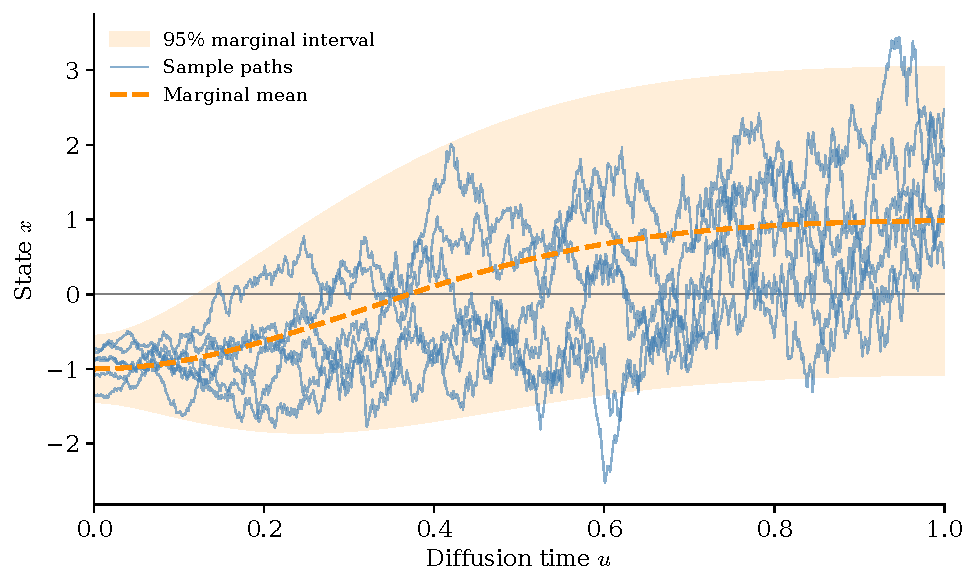
\includegraphics[width=\linewidth]{plots/gradtts/mean_reverting_sde-1.pdf}
    \caption{\textbf{1D example} A mean reverting SDE with $\bar x=0$ and $x_0=3$. The reverse process samples from a standard normal and produces $x_0=3$}
    \label{fig:mean_reverting_sde}
\end{figure}
\[
\dd\rmX = \mF(\rmX)\dd u + g(u)\dd\rmW_u
\]
\[
\dd\rmX = \left[\mF(\rmX) - g(u)^2\nabla\log p_t(\rmX)\right]\dd u + g(u)\dd\bar\rmW_u
\]
The gradient of the log-density $\nabla\log p_u(\rmX_u)$ is known as the \textit{stein score}, and models that use this are known as score-based generative models.
\[
\rmX_u=\rmM(\rmX_0,\bar\rmX,u)+\bm\varepsilon_u \qquad \bm \varepsilon_u\in\mathcal N(\bm 0,\mathsf\Sigma(u))
\]
\[
\nabla\log p_u(\rmX_u|\rmX_0)=-\mathsf\Sigma(u)^{-1}\bm\varepsilon_u
\]
\[
\Ls=\mS_\theta(\rmX_u,u) - (-\mathsf\Sigma(u)^{-1}\bm\varepsilon_u)
\]
\[
\rmX_U\sim \mathcal N (\bar\rmX,\tSigma(U)) 
\]
\[
\dd \rmX = \frac{1}{2}(\bar\rmX - \rmX_u)\beta(u) \dd u + \sqrt{\beta(u)} \dd\rmW_u
\]
\[
\dd \rmX = \left(\frac{1}{2}(\bar\rmX - \rmX_u) - \nabla\log p_u(\rmX_u)\right)\beta(u) \dd u + \sqrt{\beta(u)} \dd\hat\rmW_u
\]
\[
\dd \rmX = \left(\frac{1}{2}(\bar\rmX - \rmX_u) - \frac{1}{2}\mS_\theta(\rmX_u,u)\right)\beta(u) \dd u
\]

\section{Conditional generation}
\[
p(\rmX|\vy)=?
\]
\subsection{Classifier-free guidance}
\[
\dd \rmX = \left(\frac{1}{2}(\bar\rmX - \rmX_u) - (1 + w)\mS_\theta(\rmX_u,u|\vy) + w\mS_\theta(\rmX_u,u)\right)\beta(u) \dd u
\]

\subsection{Mean reversion with conditional score}
\[
\bar\rmX=\mE_\phi(\vy) \qquad \mS_{\theta,\phi}(\rmX,u|\vy)=\mD_\theta \left(
\begin{bmatrix}
    \rmX \\ \mE_\phi(\vy)
\end{bmatrix}
,u\right)
\]

\section{Training}

\section{Sampling with ODE solvers}
Euler sampler with step size $h$
\[
\mX_{u-h}=\mX_u -\frac{1}{2}(\bar\mX - \mX_u)\mS\beta(u)h
\]
\[
\mX_{i-1} = \mX_i - \mF_i(\mX_i)+\frac{1}{2}\tG_i\tG_i^\top\mS_\theta(\mX_i,u_i)
\]



\section{Computing likelihood}
Change of variables formula
\[
\log p_0(\rmX_0)=\log p_U(\rmX_U) +\int_0^U\nabla\cdot \mF_\theta(\rmX_u,u)\dd u
\]
Skilling-Hutchinson estimator
\[
\nabla\cdot\mF_\theta(\rmX,u)=\E_{p(\boldsymbol{\epsilon})}\left[\boldsymbol{\epsilon}^\top\nabla\mF_\theta(\rmX,u)\boldsymbol{\epsilon}\right] \quad \boldsymbol{\epsilon}\in\mathcal{N}(0,1)
\]

\[
\log p_0(\rmX_0|\vy)=?
\]
